\documentclass[%
reprint,
amsmath,amssymb,
aps,
]{revtex4-1}
\usepackage{graphicx}% Include figure files
\usepackage{dcolumn}% Align table columns on decimal point
\usepackage{bm}% bold math
\usepackage[utf8]{inputenc}
\usepackage{listings}
\usepackage{amsmath}
\usepackage{physics}
\usepackage{caption}

\makeatletter
\newcommand*{\rom}[1]{\expandafter\@slowromancap\romannumeral #1@}
\makeatother

\begin{document}
\title{Eigenvalue problems}
\author{Torstein S. Ølberg, Ada M. Veddegjerde and Oline A. Ranum}
\affiliation{%
 \textnormal{Universitetet i Oslo, Institutt for fysikk}\\
 olinear@student.matnat.uio.no : torsteol@student.matnat.uio.no
}
\date{\today}


\begin{abstract}
	The following experiment was undertaken as
\end{abstract}
\maketitle

\section*{Introduction}


\section*{Theory}


\subsection{The buckeling beam problem} \noindent 
The classical harmonic oscillator is described by the following equation of motion
\begin{equation}\label{evp}
 \frac{d^2 u(x)}{dx^2} = -k u(x)
\end{equation}
where $u(x)$ is the vertical displacement of the system in the $y$ direction. This general equation is the foundation for a large set of physical systems, for instance a spring force or the buckling beam problem. In the case of the buckling beam $k = F/\gamma$, where F is the force applied at the end of the beam in the direction towards the origin, and $\gamma$ is a constant defined by inherent properties of the beam. We will here apply the Dirichlet boundary conditions. If one defines the dimensionless variable $\rho = x/L$, L beeing the length of the beam, one can reorder the equation to
\begin{equation*}
	 \frac{d^2 u(\rho)}{d\rho^2} = -\frac{FL^2}{R} u(\rho)=-\lambda u(\rho)
\end{equation*}
This equation becomes an eigenvalue problem when discretized, on the form 
\begin{equation*}
\mathbf{A}\mathbf{x} = \lambda\mathbf{x}
\end{equation*}
Applying a Taylor approximation to the second derivative the differential equation, one writes the discretized variant as 
\begin{equation}\label{eqdis}
	-\frac{u_{i+1} -2u_i +u_{i-1} }{h^2}  = \lambda u_i
\end{equation}


\subsubsection{The analytical solution of a tridiagonal matrix}
Systems like equation \ref{eqdis} has analytical eigenpairs, as the matrix becomes a Toeplitz tridiagonal. The eigenvalues are given by the formula
\begin{equation}\label{analytical}
\lambda_j = d+2a\cos{(\frac{j\pi}{N+1})} \hspace{0.1cm} j=1,2,\dots N-1
\end{equation}


\subsection*{Eigensystem solvers} \noindent 
For a discretized systems it is possible to directly solve eigenvalue problems using similarity transformations. For instance using the Jacobi rotation method. The jacobi method transforms the matrix into a tridiagonal form using Housholder's algorithm. Given a symmetric matrix $A\in \mathbb{R}^{n\times n}$, we know that there exsists a orthogonal matrix S so that 
\begin{equation*}
	\mathbf{S}^T\mathbf{A}\mathbf{S} = \mathbf{D}
\end{equation*}
where 
\begin{equation*}
	\mathbf{D} = \begin{bmatrix}
	\lambda_1 & 0 & 0 & \dots & 0 \\
	0 & \lambda_2 & 0 & \dots & 0 \\
	\vdots & \vdots & \vdots &\vdots&\vdots\\
	0 & 0 & 0 &\dots & \lambda_n
	\end{bmatrix}
\end{equation*}
and $\lambda_i$ are the eigenvalues of $A$. Thus one can preform a series of similarity transformations on $\mathbf{A}$ in order to reduce it to a diagonal form. Matrix $\mathbf{B}$ is said to be a similarity transform of $\mathbf{A}$ if 
\begin{equation} \label{eq2}
	\mathbf{B} = \mathbf{S}^T\mathbf{A}\mathbf{S}, \hspace{3mm} \textnormal{where} \hspace{3mm} \mathbf{S}^T\mathbf{S} = \mathbf{S}^{-1}\mathbf{S} = \mathbf{I}
\end{equation}
A similarity transform yields a matrix with the same eigenvalues, but in general different eigenvectors. \\
Initially, one has the eigenvalue problem and a similarity matrix as defined in \ref{eq2}. One then subsequently apply a similarity transform so that 
\begin{equation}
	\mathbf{S}_N^T...\mathbf{S}_1^T\mathbf{A}\mathbf{S}_1...\mathbf{S}_N = \mathbf{D}
\end{equation}
Where the diagonal elements of $\mathbf{D}$ are the eigenvalues of $\mathbf{A}$, this method is better known as Jacobi's method [M. Jensen].

\subsubsection*{Jacobi's method}  \noindent 
Jacobi's method considers an $n\times n$ orthogonal transformation matrix on the form 
\begin{equation*}
\mathbf{S} = \begin{bmatrix}
1 & 0  & \dots & 0 &\vdots &0 \\
0 & 1  & \dots & 0 & \vdots & 0 \\
\vdots & \vdots &\vdots&\vdots&\vdots&\vdots\\
0 & 0 & \cos{\theta} & 0 &\vdots & \sin{\theta} \\
0  & 0 & 0 & 1 &\vdots & 0 \\
 \vdots & \vdots &\vdots&\vdots&\vdots&\vdots\\
 0 & 0 &\dots & -\sin{\theta} & \vdots & \cos{\theta}
\end{bmatrix}
\end{equation*}
where $\mathbf{S} = \mathbf{S}^-1$. This matrix makes a plane rotation of an angle $\theta$ in the Euclidean n-dimensional space. The similarity matrix is defined through the quantities $\tan\theta = t= s/c$, with $s=\sin\theta$ and $c=\cos\theta$ and
\begin{equation*}\cot 2\theta=\tau = \frac{a_{ll}-a_{kk}}{2a_{kl}}.
\end{equation*}
where $a_{kl}$ should be the largest off-diagonal matrix element in order to ensure that all other off-diagonal elements converges towards zero. The identity $\cot 2\theta=1/2(\cot \theta-\tan\theta)$ leads to the quadratic equation
\begin{equation*}
t^2+2\tau t-1= 0,
\end{equation*}
resulting in
\begin{equation*}
t = -\tau \pm \sqrt{1+\tau^2},
\end{equation*}
Where we choose the sign that minimizes t. Then $c$ and $s$ are easily obtained via
\begin{equation}\label{sc}
c = \frac{1}{\sqrt{1+t^2}} \hspace{5mm}  \textnormal{and} \hspace{5mm} s=tc
\end{equation}  

\subsection{The Jacobi Method}

\subsection{Unitary transformations} \noindent 
A unitary transformation is a transformation that preserves the orthogonality and inner product. Given a basis of vectors $\vec{v_i}$ ,
\begin{equation*}
	\mathbf{v}_i = \begin{bmatrix} v_{i1} \\ \dots \\ \dots \\v_{in} \end{bmatrix}
\end{equation*}
where the basis is orthogonal 
\begin{equation*}
	\mathbf{v}_j^T\mathbf{v}_i = \delta_{ij}
\end{equation*}
Given the unitary transformation 
\begin{equation*}
	\mathbf{w}_i=\mathbf{U}\mathbf{v}_i
\end{equation*}
It can be shown that the transformation preserves orthogonality
\begin{align*}
	\mathbf{w}=\mathbf{U}\mathbf{v} &\implies \mathbf{w}^T=\mathbf{v}^T\mathbf{U}^T \\ &\implies \mathbf{w}^T\mathbf{w} = \mathbf{v}^T\mathbf{U}^T\mathbf{U}\mathbf{v} = \mathbf{v}^T\mathbf{v} = \delta
\end{align*}
To show that it preserves the inner product we define 
\begin{align*}
	\mathbf{a} &= U\mathbf{b} \\
	\rightarrow \mathbf{a}^T &= \mathbf{b}^TU^T \\
	&\textnormal{We then take the inner product:} \\
	 \mathbf{a}^T\mathbf{w} &= \mathbf{b}^TU^TU\mathbf{v} = \mathbf{b}^T\mathbf{v}
\end{align*}
Where we have showed that the unitary transformation does not affect the inner product. 

\subsection{The Frobenius norm}
\begin{equation}
	\parallel A \parallel_F^2 = \parallel B \parallel_F^2 = \sum_{ij} \abs{a_{ij}}^2 = \sum_{ij} \abs{b_{ij}}^2
\end{equation}
The Frobenius norm is conserved under orthogonal/unitary transformations. 

\subsection{The Quantum Harmonic Oscillator} \noindent 
Another famous harmonic oscillator is the famous description of electron-electron interaction. Electrons in a three-dimensional harmonic oscillator potential will repel each other via the static Coulomb interaction. We assume spherical symmetry. For such a system, the radial part of the Schroedinger equation for one electron reads
\begin{equation*}
-\frac{\hbar^2}{2 m} \left ( \frac{1}{r^2} \frac{d}{dr} r^2
\frac{d}{dr} - \frac{l (l + 1)}{r^2} \right )R(r) 
+ V(r) R(r) = E R(r).
\end{equation*}
where V(r) is set to be the harmonic oscillator potential 
\begin{equation*}
	V(r) = \dfrac{1}{2}kr^2 = \dfrac{1}{2}m\omega^2r^2
\end{equation*}
E is the energy of the harmonic oscillator in three dimensions, and given the oscillator frequency $\omega$ the energy eigenvalues correspond to 

\begin{equation*}
E_{nl}=  \hbar \omega \left(2n+l+\frac{3}{2}\right),
\end{equation*}
with energy level $n=0,1,2,\dots$ and the orbital momentum $l=0,1,2,\dots$ of the electron. Though the usual substitution $R(r) \rightarrow u(r)/r$ and introduction of the dimensionless variable $\rho = r/\alpha$, $\alpha$ is a constant with dimension length, we get

\begin{equation*}
-\frac{\hbar^2}{2 m \alpha^2} \frac{d^2}{d\rho^2} u(\rho) 
+ \left ( V(\rho) + \frac{l (l + 1)}{\rho^2}
\frac{\hbar^2}{2 m\alpha^2} \right ) u(\rho)  = E u(\rho)
\end{equation*}
The boundary condition is given by $u(0) = u(\infty) = 0$, and the equation is further reducible by inserting the potential and set l = 0. After some shuffling of constants one gets the equation  
\begin{equation*}
-\frac{d^2}{d\rho^2} u(\rho) 
+ \frac{mk}{\hbar^2} \alpha^4\rho^2u(\rho)  = \frac{2m\alpha^2}{\hbar^2}E u(\rho) .
\end{equation*}
Where $\alpha$ is fixed to be 
\begin{equation*}
\alpha = \left(\frac{\hbar^2}{mk}\right)^{1/4}
\end{equation*}
This comes together to yield the energy eigenvalues 
\begin{equation*}
\lambda = \frac{2m\alpha^2}{\hbar^2}E,
\end{equation*}
and the Schroedinger's equation can be expressed as
\begin{equation}\label{qho}
-\frac{d^2}{d\rho^2} u(\rho) + \rho^2u(\rho)  = \lambda u(\rho)
\end{equation}
See any introductory book on quantum mechanics for for further details. [Griffiths, 2014]. 
\subsubsection{Discretizing the quantum harmonic osccilator}
Looking to the discretization of equation \ref{eqdis}, we see that it can be expanded to also cover this problem by a small modification. By including the electron-electron potential we now write 
\begin{equation}\label{eqho2}
	-\frac{u_{i+1} -2u_i +u_{i-1}}{h^2}+\rho_i^2u_i=-\frac{u_{i+1} -2u_i +u_{i-1} }{h^2}+V_iu_i  = \lambda u_i
\end{equation}
where $V_i=\rho_i^2$ is the harmonic oscillator potential. To solve this problem numerically one sets all diagonal elements to 
\begin{equation}\label{hoeq3}
d_i=\frac{2}{h^2}+V_i
\end{equation}
and set all non-diagonal matrix elements to
\begin{equation}\label{hoeq4}
e_i=-\frac{1}{h^2}
\end{equation}
By this definition the Schrodinger equation can be described as
\begin{equation*}
d_iu_i+e_{i-1}u_{i-1}+e_{i+1}u_{i+1}  = \lambda u_i,
\end{equation*}
where $u_i$ is unknown. This yields the eigenvalue problem
\begin{equation}\label{evho}
\begin{bmatrix}d_0 & e_0 & 0   & 0    & \dots  &0     & 0 \\
e_1 & d_1 & e_1 & 0    & \dots  &0     &0 \\
0   & e_2 & d_2 & e_2  &0       &\dots & 0\\
\dots  & \dots & \dots & \dots  &\dots      &\dots & \dots\\
0   & \dots & \dots & \dots  &\dots  e_{N-1}     &d_{N-1} & e_{N-1}\\
0   & \dots & \dots & \dots  &\dots       &e_{N} & d_{N}
\end{bmatrix}  \begin{bmatrix} u_{0} \\
u_{1} \\
\dots\\ \dots\\ \dots\\
u_{N}
\end{bmatrix}=\lambda \begin{bmatrix} u_{0} \\
u_{1} \\
\dots\\ \dots\\ \dots\\
u_{N}
\end{bmatrix}
\end{equation}

\subsection{The Lanczos algorithm}
The Lanczos iteration method is a method for diagonalizing symmetric matrices with huge dimensionalities. It will generate a sequence of real tridiagonal matrices $T_l$ ...

\newpage.
\newpage 

\section*{Method}
\subsection{Jacobi's method for Eigensolvers}
\noindent When implementing Jacobi's method we apply the following algorithm to a matrix A:
\begin{align*}
	&b_{ii} = a_{ii} \hspace{2mm}& i\not=k &\hspace{2mm} i\not=l\\
	&b_{ik} = a_{ik}\cos\theta -a_{il}\sin\theta \hspace{2mm}& i\not=k &\hspace{2mm} i\not=l \\
	&b_{il}  = a_{il}\cos\theta -a_{ik}\sin\theta \hspace{2mm}& i\not=k &\hspace{2mm} i\not=l\\
	&b_{kk} = a_{kk}\cos^2\theta -2a_{kl}\cos\theta\sin\theta +a_{ll}\sin^2\theta&&\\
	&b_{ll} = a_{ll}\cos^2\theta -2a_{kl}\cos\theta\sin\theta +a_{kk}\sin^2\theta&& \\
	&b_{kl} = (a_{kk}-a_{ll})\cos\theta\sin\theta+a_{kl}(\cos^2\theta -\sin^2\theta)\\
\end{align*}
where $c = \cos\theta$ and $s = sin\theta$ are defined as in equation \ref{sc}. The system of iterations are implemented in a while loop that keeps track of the norm of all the off diagonal elements. We state that when this sum is belove a threshold of $10^{-10}$, we have reduced the matrix to a diagonal form. From this form we read the eigenvalues of the matrix $\hat{D}$ across the diagonal. \\
In order to ensure that we obtained accurate results, we compare the egeinvalues produced by Jacobis method with the analytical solution produced by equation \ref{analytical}. To do so, we use an initial tridiagonal matrix where all off-diagonal are equal, and all elements across the diagonal are equal. \\
To look closer at the efficiency of the method, we compare the results agains the armadillo function for solving eigenvalue problems. We look at the time both algorithm uses, as well as the proximity to the analytical results. We test for N = 20 grid points for a 2D tridiagonal matrix.  
\subsection{Unit Testing}

\subsection{Extending the algorithm to the Quantum oscillator} \noindent 
By looking at equation \ref{qho} we see that it is almost on the same form as the equation of the buckling beam problem. In fact, it only deviates by a constant factor. Thus we make a small modification to our established algorithm in order to extend it to cover the electron-electron interaction. We next look to equation \ref{eqho2}, and define the matrix element as given by equation \ref{hoeq3} and \ref{hoeq4}. The eigenvalue problem we solve is described by equation \ref{evho}. We reuse the code from the Buckling beam problem, with the minor potential modification.

\subsection{2D:Quantum dots in three dimensions, one electron} \noindent 
We then extend our algorithm to solve for one electron in three dimensions, we do so by adding the harmonic oscillator potential to the tridiagonal Toeplitz matrix as in equation \ref{qho}. We then apply the Jacobi method to diagonalize the matrix, and read off the estimated eigenvalues of the diagonal matrix. We study the results as functions of the number of integration points N and the approximation to $\rho_{max}$. We vary N with $N\in[10, 70, 100, 200]$, for each N we vary $\rho_{max} \in [1, 2, 3, 4, 5, 6, 7, 8, 15, 100]$. We then evaluate the results by estimating the relative error as given by equation \ref{relerror}, and compare values of $\rho$ per N. After evaluating these results we set $\rho_{max} = 5$, and choose N = 100. We then take a closer look at this selection, and find the lowest value of integration points needed in order to reproduce the analytical solution with four leading digits after the decimal point. 

\newpage.
\newpage 

\section*{Results}
\begin{figure}[!h]
	\begin{tabular} {|c|c|c|c|}
		\hline
		Run & \# Transforms & Time Jacobi [s] & Time armadillo [s] \\ 
		\hline
		&&& \\ 
		1 & 19286 & 3.687817             & 0.002251            \\ 
		2 & 19286 & 3.520625             & 0.001646            \\ 
		3 & 19286 & 3.53273             & 0.001579            \\ 
		4 & 19286 & 3.51314             & 0.001565            \\ 
		5 & 19286 & 3.536378             & 0.001629            \\ 
		6 & 19286 & 3.560997             & 0.001663            \\ 
		7 & 19286 & 3.567837             & 0.001561            \\ 
		8 & 19286 & 4.936219             & 0.001647            \\ 
		9 & 19286 & 4.872346             & 0.003301            \\ 
		10 & 19286 & 3.865138             & 0.001855            \\ 
		\hline 
		& & &\\
		Average &&& \\ 
		\hline
	\end{tabular}
	\label{tab1}
	\captionof{table}[foo]{Time estimations of the Jacobi and the armadillo eig\_sym solvers to find eigenvalues of a 100$\times$100 matrix. Included the number of similarity transformations nesecarry during this run of the Jacobi method.}
\end{figure}



\subsection*{2D:Quantum dots in three dimensions, one electron}
Study the result as a function of integration points N and the approximation to 
When estimating the given values of N and $\rho_{max}$ we find the following relations in the relative error given as in figure \ref{fig:2D10}, \ref{fig:2D70}, \ref{fig:2D100} and \ref{fig:2D200} in the appendix.\\
When evaluating figure \ref{fig:2D10}, \ref{fig:2D70}, \ref{fig:2D100} and \ref{fig:2D200} we see a couple of general trends. The relative error between the estimated eigenvalues and the analytical eigenvalues has a tendency to decrease as N increases. As well, we see that there is a region around $\rho = 5$ where the relative error is the smallest. \\  
With $\rho_{max} = 5$ and N = 100 we find that it takes approximately 200 gridpoints to reproduce the analytical results with four leading digits. There is some variations in regards to what eigenvalue we are looking at. The resoults are presented in figure \ref{fig:LD}\\  

\section*{Discussion} 

\subsection*{2D: Quantum dots in three dimensions, one electron} \noindent 
It is interesting to see how the relative error varies with each choice of N and $\rho_{max}$. It is evident that the error decreases as N increases, but furthermore, they all show the same tendencies in regards to $\rho_{max}$. $\rho_{max} = 5$ for all tested values of N appears to be the value that most consistently yields the lowest error. At certain times one can see $\rho_{max} = 3$ or $\rho_{max} = 4$ yielding lower values for the lowest eigenvalues for N > 10, but in these cases they will have a rapid growth in the error. Thus we do not find them to be equally reliable with the current information. Of course, access to a broader selection of analytical eigenvalues would help us determine the quality of this information. \\
\textit{Mention something about N=10 results versus N$>$10}\\
Even though it is hard to say something certain about the eigenvalues beyond $\lambda = 11$, the error curves seems to form a distribution with around $\rho_{max} = 5$. \\
\textit{discussion of leading digets}



\section*{Conclusion}


\newpage .
\newpage 
\onecolumngrid
\section*{Bibliography}
\noindent $[1]$ Griffiths Quantum Mechanics\\ 
$[2]$
\section*{Appendix A}
For the code used for calculation our results, visit
\url{https://github.com/OlineRanum/FYS3150/Project_2}
\newpage 
\subsection{Plots}
\begin{figure*}[!h]
	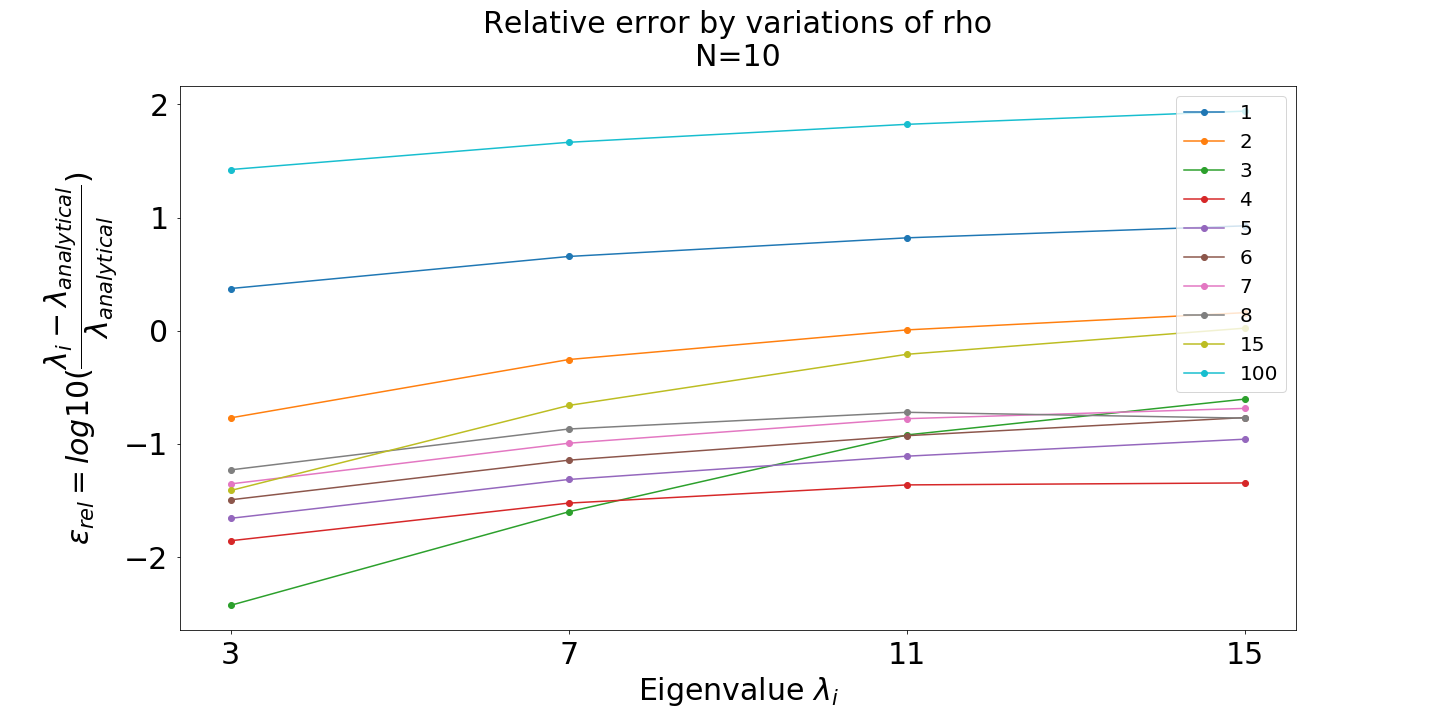
\includegraphics[scale = 0.3]{N_10_relative_error.png}
	\caption{\label{fig:2D10}}
\end{figure*}
\begin{figure*}[!h]
	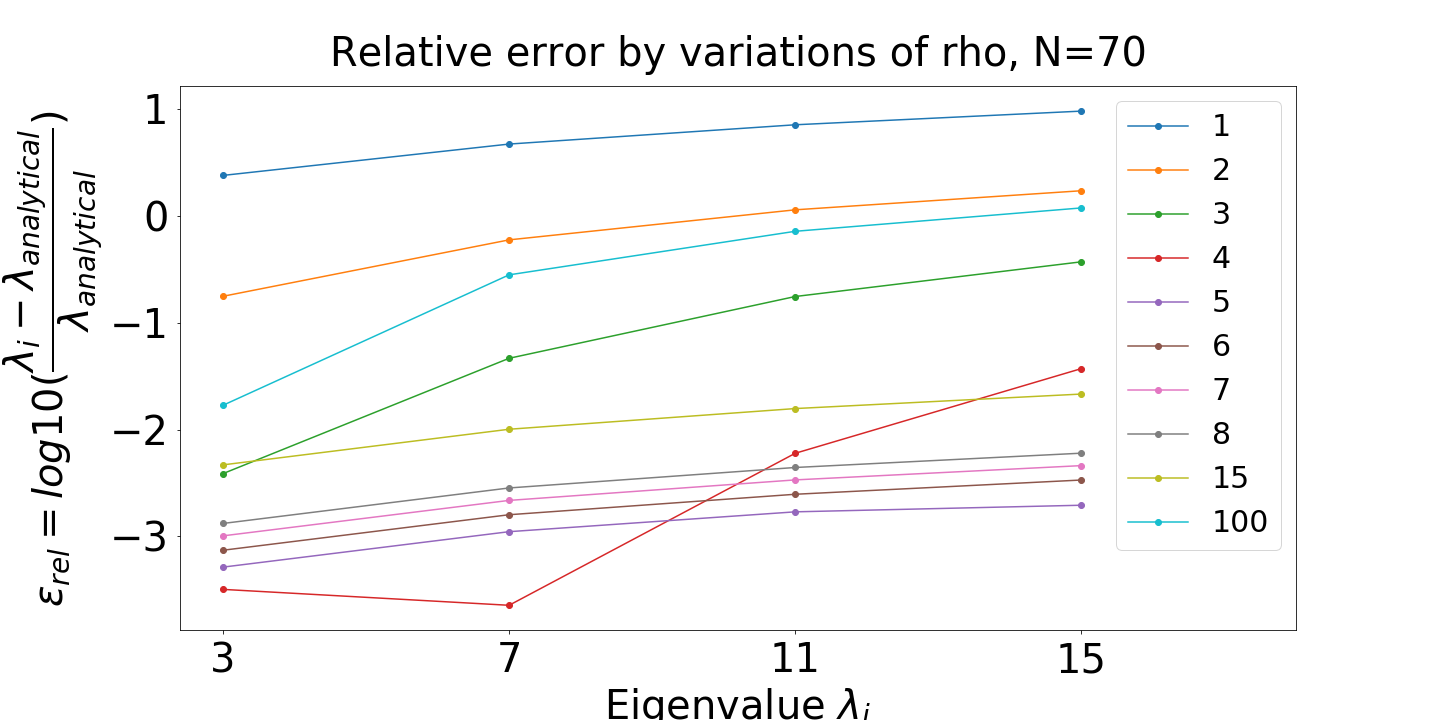
\includegraphics[scale = 0.3]{N_70_relative_error.png}
	\caption{\label{fig:2D70}}
\end{figure*}
\begin{figure*}[!h]
	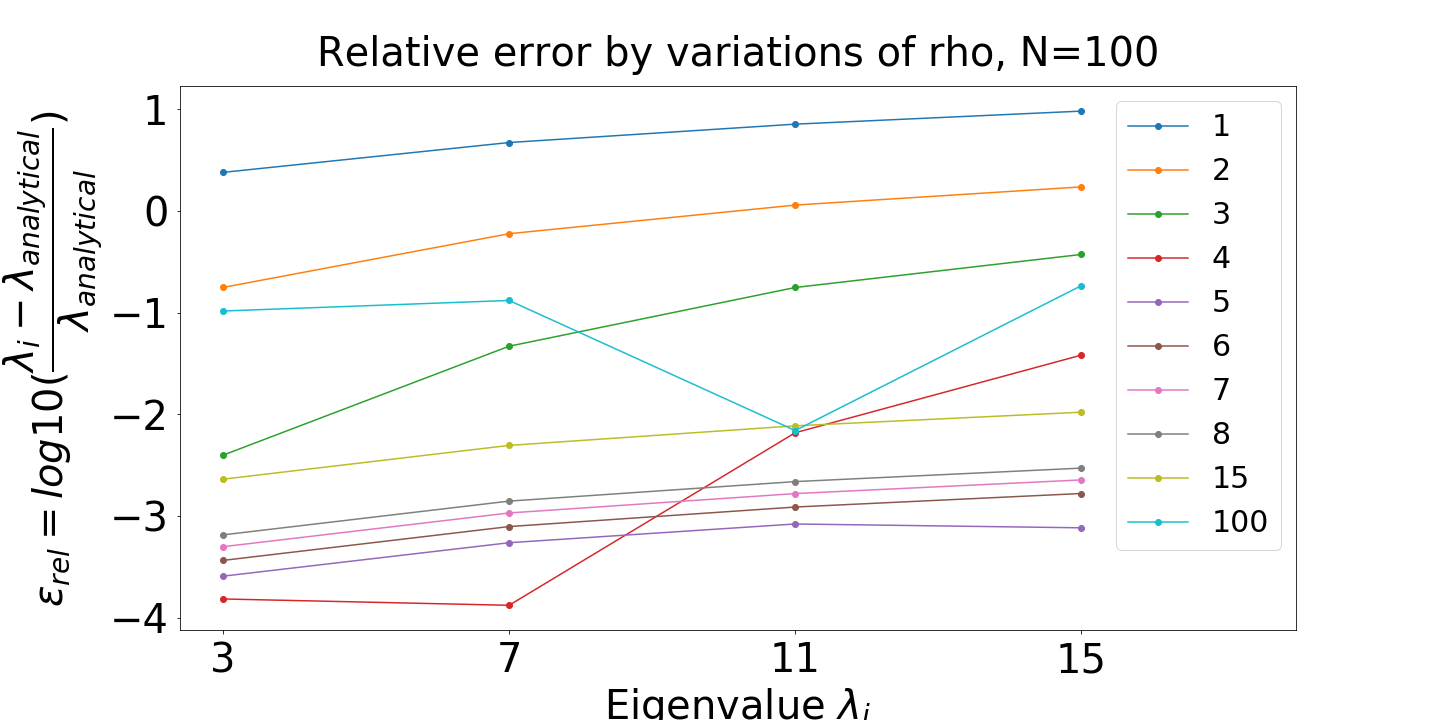
\includegraphics[scale = 0.3]{N_100_relative_error.png}
	\caption{\label{fig:2D100}}
\end{figure*}
\begin{figure*}[!h]
	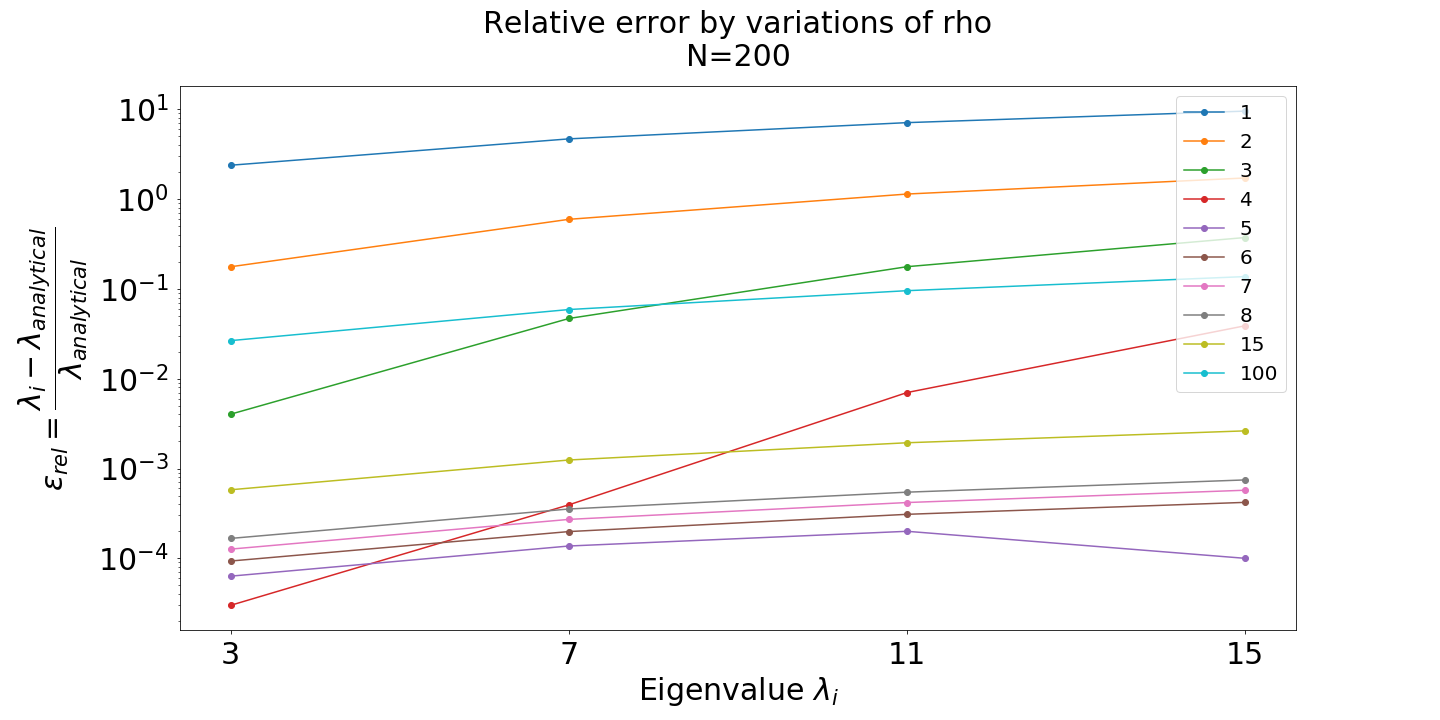
\includegraphics[scale = 0.3]{N_200_relative_error.png}
	\caption{\label{fig:2D200}}
\end{figure*}
\begin{figure*}[!h]
	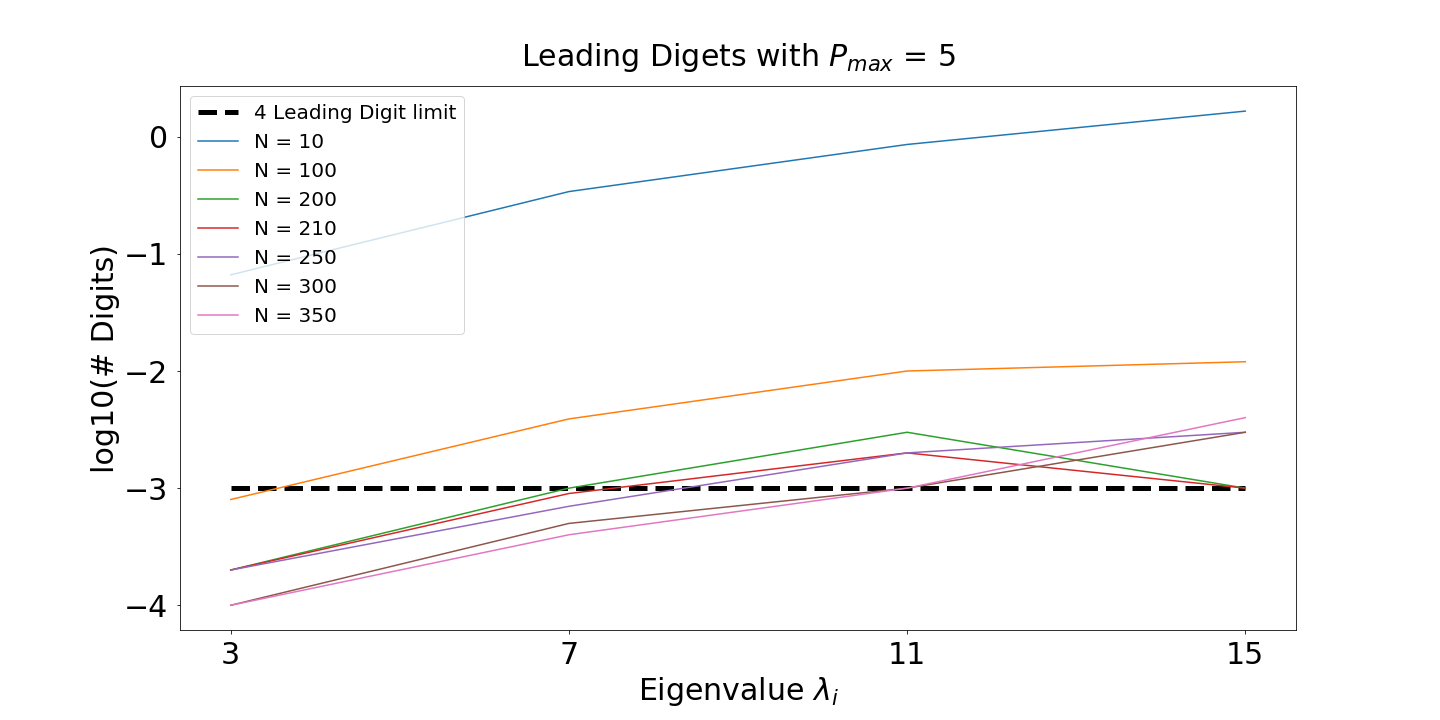
\includegraphics[scale = 0.3]{Leading_digits.png}
	\caption{\label{fig:LD} The figure show the relation between the number for leading digits, in regards to the black bar representing four leading digits.}
\end{figure*}

\end{document}